% Template for Cogsci submission with R Markdown

% Stuff changed from original Markdown PLOS Template
\documentclass[10pt, letterpaper]{article}

\usepackage{cogsci}
\usepackage{pslatex}
\usepackage{float}
\usepackage{caption}

% amsmath package, useful for mathematical formulas
\usepackage{amsmath}

% amssymb package, useful for mathematical symbols
\usepackage{amssymb}

% hyperref package, useful for hyperlinks
\usepackage{hyperref}

% graphicx package, useful for including eps and pdf graphics
% include graphics with the command \includegraphics
\usepackage{graphicx}

% Sweave(-like)
\usepackage{fancyvrb}
\DefineVerbatimEnvironment{Sinput}{Verbatim}{fontshape=sl}
\DefineVerbatimEnvironment{Soutput}{Verbatim}{}
\DefineVerbatimEnvironment{Scode}{Verbatim}{fontshape=sl}
\newenvironment{Schunk}{}{}
\DefineVerbatimEnvironment{Code}{Verbatim}{}
\DefineVerbatimEnvironment{CodeInput}{Verbatim}{fontshape=sl}
\DefineVerbatimEnvironment{CodeOutput}{Verbatim}{}
\newenvironment{CodeChunk}{}{}

% cite package, to clean up citations in the main text. Do not remove.
\usepackage{apacite}

% KM added 1/4/18 to allow control of blind submission
\cogscifinalcopy

\usepackage{color}

% Use doublespacing - comment out for single spacing
%\usepackage{setspace}
%\doublespacing


% % Text layout
% \topmargin 0.0cm
% \oddsidemargin 0.5cm
% \evensidemargin 0.5cm
% \textwidth 16cm
% \textheight 21cm

\title{Exploring potential gender stereotypes in the distributional
semantics of child-directed speech}

\usepackage{booktabs}
\usepackage{longtable}
\usepackage{array}
\usepackage{multirow}
\usepackage{wrapfig}
\usepackage{float}
\usepackage{colortbl}
\usepackage{pdflscape}
\usepackage{tabu}
\usepackage{threeparttable}
\usepackage{threeparttablex}
\usepackage[normalem]{ulem}
\usepackage{makecell}
\usepackage{xcolor}

\author{{\large \bf Benjamin E. deMayo (bdemayo@princeton.edu)} \\ Princeton University}

\newlength{\cslhangindent}
\setlength{\cslhangindent}{1.5em}
\newenvironment{CSLReferences}%
  {}%
  {\par}

\begin{document}

\maketitle

\begin{abstract}
Abstract: In three analyses, I explore whether gender stereotypes might
be present in the distributional semantics of the CHILDES corpus
(MacWhinney 2000), a large compendium of transcribed conversations
between caregivers and their children, by training 2 commonly-used word
embedding models on the corpus. In the first analysis, I examine the
correlation between the gender valence of individual word vector
representations in the two word-embedding models. In the second
analysis, I relate gender valence in the word vector representations of
individual words to human ratings of those words' gender valence. In the
third analysis, I examine whether specific stereotypical associations
with gender are detectable in the vector space representation of the
words.

\textbf{Keywords:}
gender bias; word-embedding models; distributional semantics.
\end{abstract}

\hypertarget{introduction}{%
\section{Introduction}\label{introduction}}

Gender is a highly salient social category that develops within the
first few years of life and maintains its importance across the lifespan
(Ruble, Martin, \& Berenbaum, 2006). Gender stereotypes, characteristics
that are believed to be true of a gender category as a whole, are most
rigid in middle childhood (around ages 5-8), but their developmental
roots are in early childhood (Halim \& Ruble, 2010). How children form
concepts of gender, as well as the stereotypes that are linked to those
concepts, has long been a subject of research, with some researchers
proposing that language input to children could have a consequential
impact on children's beliefs about gender categories.

Broadly speaking, two theoretical approaches have attempted to explain
how language input to children might shape their gender stereotypes. One
approach has emphasized the communication of knowledge from adults to
children in a ``top-down'' fashion, in which children hear statements
that explicitly communicate information about groups, such as generic
statements (e.g., {``girls are good at reading''}; Gelman, Ware, \&
Kleinberg, 2010). Another approach, which I focus on here, emphasizes
how children could pick up on subtle cues about gender concepts and
stereotypes solely from the statistics of their language input. In other
words, children could learn that words corresponding to particular
activities, traits, occupations, and other characteristics are
themselves gendered by virtue of the other words with which they
co-occur. This latter approach shares an intimate link with the
computational linguistic subfield of distributional semantics, which
seeks to characterize how the meaning of linguistic items is related to
how those items are distributed in large bodies of text.

Several studies have leveraged the tools of distributional semantics to
examine whether gender stereotypes are appreciable in natural language
corpora; some of these studies focus specifically on language that would
likely be heard by children. The general strategy used by these studies
has involved taking large bodies of text {[}usually those with several
million tokens, though this has not always been the case; Lewis,
Borkenhagen, Converse, Lupyan, \& Seidenberg (2020){]} and using them to
train word embedding models, which generate representations of
individual word types in a high-dimensional vector space based on each
word type's co-occurrence with other types. The key assumption in such a
strategy is that words which frequently co-occur will have similar
meanings. Once vector representations of words are obtained, cosine
distances between individual lexical items in the vector space are
calculated as a proxy of semantic similarity, allowing researchers to
examine whether words' vector representations show patterns of
similarity that might be expected given prevalent societal stereotypes
(e.g., that the word ``doll'' is closer to the word ``girl'' than it is
to the word ``boy''). This general analytic framework has been used to
argue that gender stereotypes are present in the distributional
structure of large bodies of naturalistic text, including web-based
corpora, children's books, and transcripts of films and television shows
(Bhatia \& Bhatia, 2021; Caliskan, Bryson, \& Narayanan, 2017;
Charlesworth, Yang, Mann, Kurdi, \& Banaji, 2021; Lewis \& Lupyan,
2020).

In this work, I extend prior findings by examining the human-like
gender-stereotypical biases that might emerge in the vector
representations obtained from training word embedding models on a body
of child-directed speech. Specifically, I use transcripts between
caregivers and children between the ages of 1 and 3 years old from the
North American English corpora in the Child Language Data Exchange
System (CHILDES; MacWhinney, 2000) and extract vector-space semantic
representations using 2 commonly-used word embedding models, Word2Vec
(Mikolov, Chen, Corrado, \& Dean, 2013) and GloVe (Pennington, Socher,
\& Manning, 2014).

\hypertarget{method}{%
\section{Method}\label{method}}

\hypertarget{data-preprocessing}{%
\subsection{Data preprocessing}\label{data-preprocessing}}

Child-directed language was sourced from all of the North American
English transcripts in the CHILDES corpus (MacWhinney, 2000).
Transcripts were obtained using the \texttt{childes-db} API, which
allows researchers to access utterances in a tabular format that
includes metadata about each utterance, including its speaker's role
(parent, grandparent, child, etc.), the gender of the child in the
conversation, and the lemmatized ``stem'' of the utterance (Sanchez et
al., 2019). From this tabular data, the stems of utterances from
mothers, fathers, grandparents and adults were extracted and
concatenated to create the training data, which contained text from
conversations to 1,156 children, and was comprised of 6,824,349 word
tokens.

\hypertarget{word-embedding-model-training}{%
\subsection{Word embedding model
training}\label{word-embedding-model-training}}

Two common word embedding models were used to obtain vector-space
representations for words in CHILDES. The first was Word2Vec (Mikolov et
al., 2013), which uses a 2-layer neural network to predict a given word
in a sentence given its surrounding words (continuous bag of words
approach, CBOW) or vice versa (skip-gram approach) and derives
vector-space representations of each word based on the neural network
weights between the input layer and the single hidden layer of the
network. The second was GloVe (Pennington et al., 2014), an unsupervised
learning algorithm which takes as input a sparse matrix encoding the
co-occurrence frequency of each pair of lexical items in a corpus, and
which learns vector representations for these items, such that the inner
product between two vectors closely approximates a logarithmic
transformation of the probability that those two lexical items co-occur
in the text. For our purposes here, the two techniques have the same
goal of extracting vector representations of words that are semantically
meaningful, even though GloVe's learning strategy emphasizes global
co-occurrence probability between pairs of words more than Word2Vec,
which can be seen as centering more on the local semantic contexts that
words appear in. In the following analyses, the context window of each
word embedding model is set to 5 words in both directions from a target
word, and word representations derived from GloVe and Word2Vec are
vectors in a 50-dimensional space.

\hypertarget{analyses}{%
\section{Analyses}\label{analyses}}

\hypertarget{analysis-1-broad-comparison-between-word2vec-and-glove}{%
\subsection{Analysis 1: Broad comparison between Word2Vec and
GloVe}\label{analysis-1-broad-comparison-between-word2vec-and-glove}}

The first, and most broad, analysis is a coarse indication of whether
Word2Vec and GloVe are capturing roughly similar semantic information
for words in the CHILDES corpus, specifically as it concerns individual
words' gender valence. Here, I define \emph{gender valence} as the
degree which a word is either semantically closer to the concept `boy'
versus the concept `girl.' This conceptualization of gender valence has
a intuitive implementation with word embeddings: gender valence can be
thought of as a word's average cosine similarity to one or more
``anchor'' words representing the concept `girl,' minus the word's
similarity to one or more ``anchor'' words representing the concept
`boy.' For this analysis and those subsequent, anchor words were
borrowed from Lewis et al. (2020) and were as follows:
\(\text{girl words} = \{{\text{girl, woman, sister, she, her, daughter}}\}\);
\(\text{boy words} = \{{\text{boy, man, brother, he, him, son}}\}\). For
each word vector obtained from both GloVe and Word2Vec, we can calculate
this average cosine distance to the set of anchor words representing the
broader concepts of ``boy'' and ``girl.'' Importantly, the simplicity of
this analytic strategy belies the fact that words, concepts, and people
can all be high (or low) in \emph{both} masculine and feminine
characteristics, suggesting that this method is a somewhat crude, if
convenient, way of conceptualizing gender valence in lexical items.

\begin{CodeChunk}
\begin{figure}[h]

{\centering 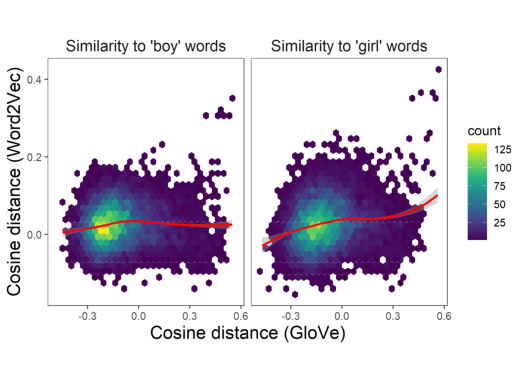
\includegraphics{figs/corr_plot-1} 

}

\caption[Hexbin plot showing association between gender valence of individual words vectors in Word2Vec and GloVe]{Hexbin plot showing association between gender valence of individual words vectors in Word2Vec and GloVe. Red lines are LOESS smoothing with 95 percent confidence intervals.}\label{fig:corr_plot}
\end{figure}
\end{CodeChunk}

To get a rough sense of whether both models are similarly capturing
semantic information related to gender, we can plot the average cosine
distance to the anchor words from both models on opposing axes (Figure
\ref{fig:corr_plot}). In both similarity to the `girl' anchor words and
similarity to the `boy' anchor words, the models show a slight positive
association where the density of points is highest; however, this
relationship is not discernible for words with more extreme values of
similarity to the anchor words. In addition, a positive correlation
between similarity metrics from the two models is more appreciable when
measuring individual words' similarity to the `girl' anchor words (right
panel of Figure \ref{fig:corr_plot}) compared to the `boy' anchor words.
The slight positive association seen in Figure \ref{fig:corr_plot},
indicates that while the two models do seem to capture some of the same
gender valence information, there is also substantial variation between
the models.

\hypertarget{analysis-2-correspondence-with-human-ratings-of-word-gender-valence}{%
\subsection{Analysis 2: Correspondence with human ratings of word gender
valence}\label{analysis-2-correspondence-with-human-ratings-of-word-gender-valence}}

Are word embedding models capturing an aspect of individual words'
gender valence that corresponds with human intuitions about how gendered
those words are? To examine this question, I computed each word's gender
valence with the same strategy as in Analysis 1.

To examine whether this quantity captures information about words that
accords with human intuitions about how ``boyish'' or ``girlish'' a word
is, I use gender judgments of over 2,000 word types by human raters from
Amazon Mechanical Turk, originally collected by Lewis et al. (2020).
Each word was rated by approximately 7 participants, and ratings fall on
a 1-5 scale, with 1 indicating that a word is as male-typed as possible
and 5 indicating that a word is as female-typed as possible. The number
of words for which this dataset contains human ratings is far less than
the number of word types present in CHILDES, so a correlation between
the word-vector similarity quantity previously mentioned and the human
ratings is only possible for a small subset of the CHILDES word types.

\begin{CodeChunk}
\begin{figure}[h]

{\centering 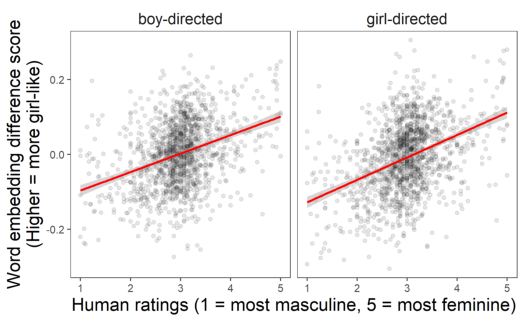
\includegraphics{figs/human_plot-1} 

}

\caption[Scatter plot showing individual words' gender valence, as determined by human raters (horizontal axis) against word embedding difference score (vertical axis)]{Scatter plot showing individual words' gender valence, as determined by human raters (horizontal axis) against word embedding difference score (vertical axis). Lines are best linear fits with associated 95 percent confidence intervals.}\label{fig:human_plot}
\end{figure}
\end{CodeChunk}

\begin{CodeChunk}
\begin{figure*}[h]

{\centering 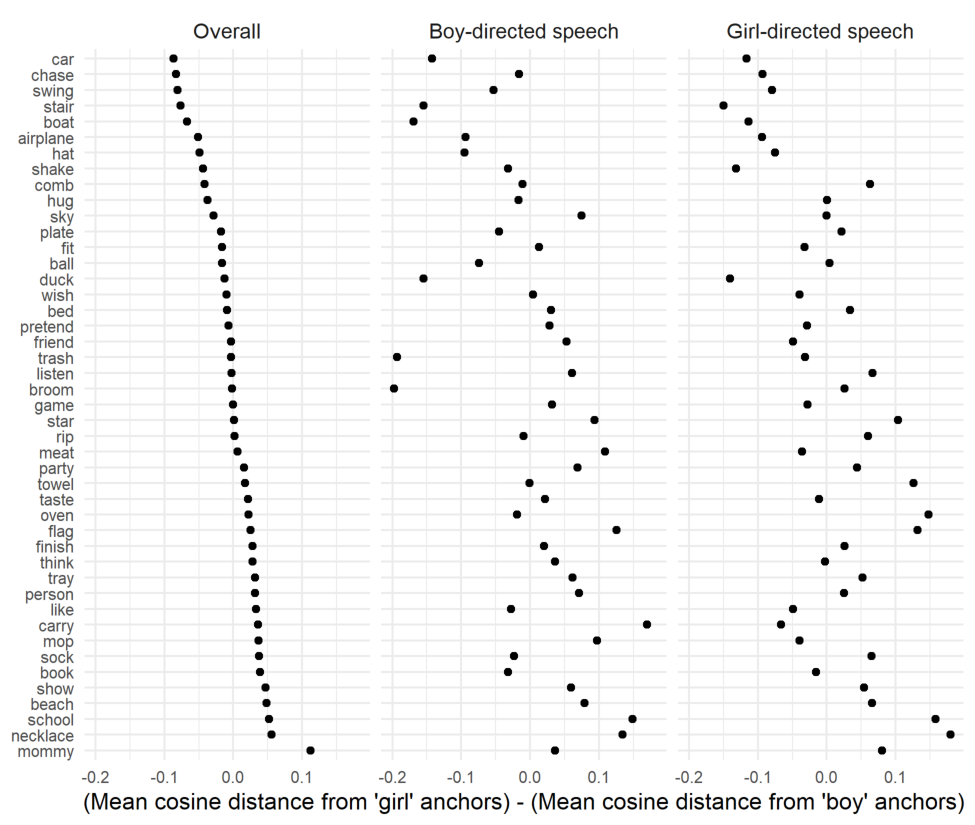
\includegraphics{figs/cdiplot-1} 

}

\caption[Gender valence of word vector representations of 45 words from the MacArthur-Bates Communicative Development Inventory Short Form]{Gender valence of word vector representations of 45 words from the MacArthur-Bates Communicative Development Inventory Short Form. Horizontal axis represents, for each word on the vertical axis, the difference between (a) the mean cosine similarity to the 'girl' anchors and (b) mean cosine similarity to the set of 'boy' anchors.}\label{fig:cdiplot}
\end{figure*}
\end{CodeChunk}

Additionally, for this analysis, two separate Word2Vec models were
trained: one on speech from CHILDES that was directed at male children,
and another on speech from CHILDES directed at female children, to
examine if communication to children of different genders shows more or
less correspondence with human intuitions about gender valence. Figure
\ref{fig:cdiplot} shows how these two models, in addition to the one
trained on all child-directed utterances (regardless of the child's
gender), represent the gender valence of 45 nouns and verbs selected
from the MacArthur-Bates Communicative Development Inventory Short Form
(Fenson et al., 2000), a language development assessment used with
children between the ages of 16 and 30 months. One noticeable pattern
from Figure \ref{fig:cdiplot} is that word vectors with higher
male-valence - at least in the model trained on all of the
child-directed utterances - tend to be modes of transportation, while
more female-valenced words tend to be articles of clothing, jewelry, and
domestic household items.

The results of the word vector correlations with human ratings are
displayed in Figure \ref{fig:human_plot}. Word embedding models trained
either on only speech to girls or speech to boys both capture
information about individual words' gender valence that shows a reliable
positive association with human ratings of a word's gender valence
(\(r_\text{girl-directed speech} =\) 0.4001;
\(r_\text{boy-directed speech}=\) 0.3514). The correlations between
human judgments and word embedding difference scores underscore two
points. First, the gendered nature of certain words, as intuited by
human raters, is discernible in the distributional semantics of language
directed to children. Second, according to the (very coarse)
correlational measure described above, this gender valence of individual
words in child-directed speech does not look radically different between
speech directed to boys vs.~girls, though other analytic strategies
could potentially still detect differences in how gendered language is
communicated to boys vs.~girls, if such differences exist.

\hypertarget{analysis-3-specific-gender-stereotypes}{%
\subsection{Analysis 3: Specific gender
stereotypes}\label{analysis-3-specific-gender-stereotypes}}

Does child-directed speech in the CHILDES corpus contain specific gender
stereotypes? In Analysis, 3, I examined whether word vector
representations derived from CHILDES encode semantic information that
encapsulates three particular stereotypes which have been the subject of
prior research in social psychology: (1) Female as home-oriented, male
as work-oriented; (2) Female as good, male as bad; and (3) Female as
oriented towards reading and language, and male as math-oriented. To
assess the extent to which these stereotypes might surface in the
distributional semantics of the CHILDES corpus, the Word Embedding
Association Test {[}WEAT; Caliskan et al. (2017){]} was conducted. The
goal of the WEAT is to quantify stereotypical biases in large bodies of
text in a manner analogous to how the Implicit Association Test
quantifies implicit bias in people (Greenwald, McGhee, \& Schwartz,
1998).

\begin{table}

\caption{\label{tab:xtable}Words for each attribute set.}
\centering
\begin{tabular}[t]{l>{\raggedright\arraybackslash}p{2in}}
\toprule
Attribute & Words\\
\midrule
Home & \{family, children, home, cousin, parent, wedding\}\\
Work & \{job, work, money, office, business, desk\}\\
Language & \{book, read, write, letter, spell, story\}\\
Math & \{number, count, sort, size, shape, different\}\\
Good & \{good, happy, gift, sunshine, heaven\}\\
\addlinespace
Bad & \{bad, awful, sick, trouble, hurt\}\\
\bottomrule
\end{tabular}
\end{table}

Defined more precisely, as in Caliskan (2017), we can consider two
equally-sized sets of anchor words \(X\) and \(Y\) (for example, the
sets corresponding to the anchor words for `boy' and `girl') and two
sets of attribute words \(A\) and \(B\) (for example, sets of words
corresponding to the attributes `good at reading' and `good at math').
The effect size generated by the WEAT is
\[\frac{\text{mean}_{x \in X}s(x, A, B) - \text{mean}_{y \in Y}s(y, A, B)}{\text{std dev}_{w \in X \cup Y}s(w, A, B)}\]
where
\[s(w, A, B) = \text{mean}_{a \in A}\text{cos}(\vec{w}, \vec{a}) - \text{mean}_{b \in B}\text{cos}(\vec{w}, \vec{b})\]

\begin{CodeChunk}
\begin{figure}[h]

{\centering 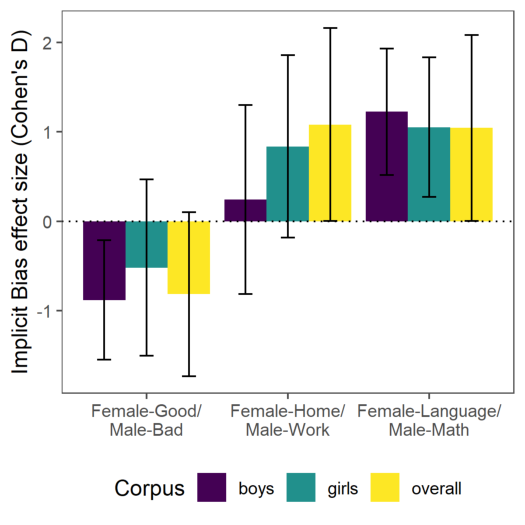
\includegraphics{figs/weatplot-1} 

}

\caption[WEAT effect sizes for each stereotype]{WEAT effect sizes for each stereotype. Error bars are 95 percent confidence intervals on effect size estimates, generated by randomly shuffling target word vector labels and simulating the WEAT effect size 1000 times.}\label{fig:weatplot}
\end{figure}
\end{CodeChunk}

For each of the three previously mentioned stereotypes, a WEAT score was
computed using 3 Word2Vec embeddings: one trained only on boy-directed
speech, one directed only on girl-directed speech, and one trained on
both. The words in each attribute set are displayed in Table 1 and were
borrowed from Lewis et al.~(2020).

Results from the WEAT test are displayed in Figure \ref{fig:weatplot}.
Ninety-five percent confidence intervals were generated for WEAT effect
size estimates by randomly shuffling which target words corresponded
with the ``boy'' concept and which with the ``girl'' concept, and
subsequently computing a WEAT effect size with the shuffled word labels
1,000 times to obtain an empirical null distribution (following the
strategy used in Charlesworth et al., 2020). For the
Female-Good/Male-Bad stereotype, WEAT computed on the CHILDES data
showed an effect associating `girl' with `bad' and `boy' with `good,'
which is in the opposite direction from what is considered stereotypical
in prior literature (Cvencek, Meltzoff, \& Greenwald, 2011). However,
only the effect size generated from speech directed to boys had an
effect size estimate whose 95\% confidence interval did not include
zero. The Female-Home/Male-Work stereotype only showed an effect whose
95\% interval did not include zero with a word embedding model trained
on speech to both boys and girls; the boy-directed and girl-directed
corpora yielded smaller and less robust effects, though all were in the
stereotypically-expected direction. The Female-Reading/Male-Math
stereotype showed, overall, the largest effect sizes across all three
training sets, with all of the three having confidence intervals that
did not include zero.

As demonstrated in Figure \ref{fig:weatplot}, the results from WEAT on
the three CHILDES corpora (all child-directed speech, boy-directed
speech, and girl-directed speech) are somewhat mixed. Many of the WEAT
calculations generated relatively large effect sizes, but large variance
in the empirical null distribution of effect sizes, resulting in wide
confidence intervals on the effect size estimates, constrains the
interpretation of above data. Nonetheless, some gender stereotypes are
discernible in the distributional semantics of the CHILDES corpus,
particularly the stereotype that associates boys with math and girls
with reading/language.

\hypertarget{discussion}{%
\section{Discussion}\label{discussion}}

In this paper, I explored the potential presence of gender stereotypes
in the distributional semantics of child-directed speech across three
analyses using the CHILDES corpus (MacWhinney, 2000). In the first
analysis, I compared how two commonly-used word embedding models, GloVe
and Word2Vec, capture the gender valence of the same words. Figure
\ref{fig:corr_plot} shows that the measure of gender valence that the
two models generate are (at most) modestly correlated. In the second
analysis, I obtained two additional sets of word vector representations
by training Word2Vec on (a) just speech to girls and (b) just speech to
boys (Figure \ref{fig:cdiplot}), and correlated the models' estimates of
individual words' gender valence to human-generated judgments(Figure
\ref{fig:human_plot}). The correlation seen in Figure
\ref{fig:human_plot} analysis demonstrates that Word2Vec, trained on
child-directed speech, to some extent captures humans' intuitions about
the gender valence of particular words. In the third analysis, I used an
existing measure of gender stereotyping in large bodies of text, the
Word Embedding Association Test, to quantify whether specific gender
stereotypes are present in child-directed speech. Figure
\ref{fig:weatplot} illustrates that specific gender stereotypes were
captured by Word2Vec, but inconsistently so. The
Female-Language/Male-Math stereotype appeared to be the most robust
effect, while the Female-Good/Male-Bad effect was in the opposite
direction from the predicted result based on past literature. Moreover,
across all three stereotypes, the empirical null distribution generated
by randomly permuting which anchor words referred to the `boy' and
`girl' categories had large variance, constraining a strong
interpretation of the effect sizes observed from the WEAT.

Given the results seen here, it is difficult to clearly explain whether
and how language directed to boys differs from language directed to
girls in terms of how much gender stereotypical information is
communicated to children. The discrepant pattern between the panels of
Figure \ref{fig:cdiplot} indicates that there was substantial
variability in individual words' gender valence as captured by Word2Vec
depending on whether the model was trained on girl-directed
vs.~boy-directed speech. In future work, one potential approach to
better understand whether the speech to boys vs.~girls contains
differing stereotype content is to examine the frequency of certain
words that have a strong gender valence in girl-directed and
boy-directed speech, similar to the approach in Braginsky, Meylan, \&
Frank (2016). A qualitative analysis of when and in what context these
very gendered words appear might also explain potential differences in
boy-directed vs.~girl-directed speech.

Training a word embedding model on child-directed utterances from
CHILDES - and then subsequently trying to use those word embeddings to
gain insight into parent-child communication - carries some inherent
limitations. First, CHILDES contains conversations between parents and
children in which children actively shape the communicative interaction.
In this paper, I excised all words spoken by children when preparing the
training data; in doing so, some information is lost about how highly
gendered speech enters into communication between caregivers and
children. Training a word embedding model on the text from one side of a
two-sided conversation is also methodologically problematic, since it
forces some constraints on the definition of what it means for one word
to be ``in the context'' of another. In this paper, I concatenated all
of the adult utterances, which forces some words to be side-by-side in
the training data when, in actual conversation, they were separated by a
child utterance. One potential solution is to adjust how the model
considers which words are in the context of any other given word, by not
extending the context window beyond the immediate conversational turn a
word appears in. This is also an imperfect solution, however, because
live conversation often includes distinct utterances that are
interrupted by other speakers or are distributed across several
conversational turns.

These methodological challenges notwithstanding, there are several
interesting directions for future research that employ similar
methodology to the current work. This paper did not consider how
language to children changes across development. Might caregivers
communicate about gender differently depending on the age of their
child? Examining whether the gender valence of particular word vectors
changes systematically over development could offer some insight on this
question. Additionally, comparing the vector-space representation of
words in CHILDES with pre-trained Word2Vec and GloVe vectors would
potentially help clarify how gendered we would expect certain words to
be in a much larger, more linguistically and contextually heterogeneous
corpus, and thus provide a useful reference point for the gendered
information we see captured in the word embedding models trained on
CHILDES. Moreover, state-of-the-art language models are able to encode
semantic information of significantly more complexity than the tools
used in these analyses, including sentence-level contextual information
(e.g., Devlin, Chang, Lee, \& Toutanova, 2018). Investigating the extent
to which these models learn gender biases and stereotypes based on
child-directed speech is an exciting possibility for future research,
but would require substantially larger corpora of child-directed speech
than CHILDES.

Returning to the question of how exactly children learn gender biases
and stereotypes, my results here suggest that child-directed speech may
indeed subtly shape children's gendered associations with traits,
activities, and objects, simply by virtue of the distributional
semantics of the speech they hear. The results here are, however, also
mixed; future investigations with larger datasets - and more power to
understand how caregivers' communication about gender might vary across
development - are needed to understand the extent to which
distributional semantics of child-directed speech shape gender biases
and stereotypes.

\hypertarget{acknowledgements}{%
\section{Acknowledgements}\label{acknowledgements}}

Thanks to Dan Friedman and Zaid Zada for guidance on this project, and
to Kyle MacDonald for his RMarkdown CogSci tools.

\hypertarget{references}{%
\section{References}\label{references}}

\setlength{\parindent}{-0.1in} 
\setlength{\leftskip}{0.125in}

\noindent

\hypertarget{refs}{}
\begin{CSLReferences}{1}{0}
\leavevmode\vadjust pre{\hypertarget{ref-bhatia2021changes}{}}%
Bhatia, N., \& Bhatia, S. (2021). Changes in gender stereotypes over
time: A computational analysis. \emph{Psychology of Women Quarterly},
\emph{45}(1), 106--125.

\leavevmode\vadjust pre{\hypertarget{ref-braginsky2016gender}{}}%
Braginsky, M., Meylan, S., \& Frank, M. C. (2016). Gender differences in
lexical input and acquisition. In \emph{41st annual boston university
conference on language development (BUCLD)}.

\leavevmode\vadjust pre{\hypertarget{ref-caliskan2017semantics}{}}%
Caliskan, A., Bryson, J. J., \& Narayanan, A. (2017). Semantics derived
automatically from language corpora contain human-like biases.
\emph{Science}, \emph{356}(6334), 183--186.

\leavevmode\vadjust pre{\hypertarget{ref-charlesworth2021gender}{}}%
Charlesworth, T. E., Yang, V., Mann, T. C., Kurdi, B., \& Banaji, M. R.
(2021). Gender stereotypes in natural language: Word embeddings show
robust consistency across child and adult language corpora of more than
65 million words. \emph{Psychological Science}, \emph{32}(2), 218--240.

\leavevmode\vadjust pre{\hypertarget{ref-cvencek2011math}{}}%
Cvencek, D., Meltzoff, A. N., \& Greenwald, A. G. (2011). Math--gender
stereotypes in elementary school children. \emph{Child Development},
\emph{82}(3), 766--779.

\leavevmode\vadjust pre{\hypertarget{ref-devlin2018bert}{}}%
Devlin, J., Chang, M.-W., Lee, K., \& Toutanova, K. (2018). Bert:
Pre-training of deep bidirectional transformers for language
understanding. \emph{arXiv Preprint arXiv:1810.04805}.

\leavevmode\vadjust pre{\hypertarget{ref-fenson2000short}{}}%
Fenson, L., Pethick, S., Renda, C., Cox, J. L., Dale, P. S., \& Reznick,
J. S. (2000). Short-form versions of the MacArthur communicative
development inventories. \emph{Applied Psycholinguistics}, \emph{21}(1),
95--116.

\leavevmode\vadjust pre{\hypertarget{ref-gelman2010effects}{}}%
Gelman, S. A., Ware, E. A., \& Kleinberg, F. (2010). Effects of generic
language on category content and structure. \emph{Cognitive Psychology},
\emph{61}(3), 273--301.

\leavevmode\vadjust pre{\hypertarget{ref-greenwald1998measuring}{}}%
Greenwald, A. G., McGhee, D. E., \& Schwartz, J. L. (1998). Measuring
individual differences in implicit cognition: The implicit association
test. \emph{Journal of Personality and Social Psychology}, \emph{74}(6),
1464.

\leavevmode\vadjust pre{\hypertarget{ref-halim2010gender}{}}%
Halim, M. L., \& Ruble, D. (2010). Gender identity and stereotyping in
early and middle childhood. In \emph{Handbook of gender research in
psychology} (pp. 495--525). Springer.

\leavevmode\vadjust pre{\hypertarget{ref-lewis2020might}{}}%
Lewis, M., Borkenhagen, M. C., Converse, E., Lupyan, G., \& Seidenberg,
M. S. (2020). What might books be teaching young children about gender?

\leavevmode\vadjust pre{\hypertarget{ref-lewis2020gender}{}}%
Lewis, M., \& Lupyan, G. (2020). Gender stereotypes are reflected in the
distributional structure of 25 languages. \emph{Nature Human Behaviour},
\emph{4}(10), 1021--1028.

\leavevmode\vadjust pre{\hypertarget{ref-macwhinney2000childes}{}}%
MacWhinney, B. (2000). \emph{The CHILDES project: The database} (Vol.
2). Psychology Press.

\leavevmode\vadjust pre{\hypertarget{ref-mikolov2013efficient}{}}%
Mikolov, T., Chen, K., Corrado, G., \& Dean, J. (2013). Efficient
estimation of word representations in vector space. \emph{arXiv Preprint
arXiv:1301.3781}.

\leavevmode\vadjust pre{\hypertarget{ref-pennington2014glove}{}}%
Pennington, J., Socher, R., \& Manning, C. D. (2014). GloVe: Global
vectors for word representation. In \emph{Empirical methods in natural
language processing (EMNLP)} (pp. 1532--1543). Retrieved from
\url{http://www.aclweb.org/anthology/D14-1162}

\leavevmode\vadjust pre{\hypertarget{ref-ruble2006gender}{}}%
Ruble, D. N., Martin, C. L., \& Berenbaum, S. A. (2006). Gender
development.

\leavevmode\vadjust pre{\hypertarget{ref-sanchez2019childes}{}}%
Sanchez, A., Meylan, S. C., Braginsky, M., MacDonald, K. E., Yurovsky,
D., \& Frank, M. C. (2019). Childes-db: A flexible and reproducible
interface to the child language data exchange system. \emph{Behavior
Research Methods}, \emph{51}(4), 1928--1941.

\end{CSLReferences}

\bibliographystyle{apacite}


\end{document}
